\section{Produktübersicht}
\setboolean{@twoside}{false}


\subsection{Systemarchitektur}

\begin{figure}[h]
	\centering
	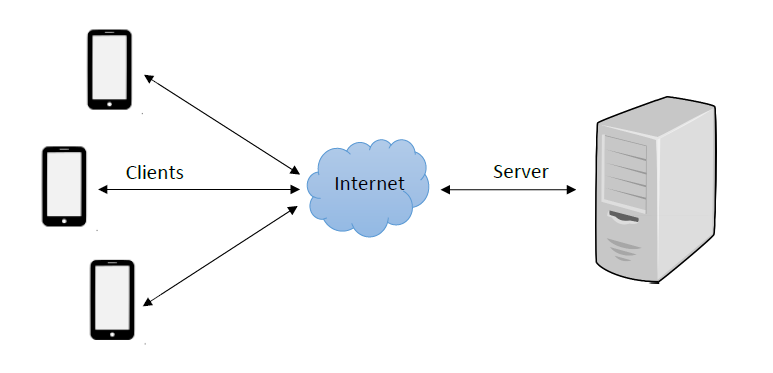
\includegraphics[scale = 0.8]{res/clientServerArchitektur.png}
\end{figure}

Mobiltelefone auf denen die Go-App läuft, müssen unter anderem zur Gruppenverwaltung
und Positionsübermittlung Daten austauschen.
Im heutigen Internet wird jedoch aufgrund der IPv4-Knappheit vermehrt Network Address Translation (NAT)
eingesetzt die einen direkten Datenaustausch verhindert. Zudem sind Endgeräte häufig durch Firewalls vor Zugriffen
von außen geschützt.
Insbesondere Mobiltelefone sind häufig von diesen Problemen betroffen.

Um dem zu begegnen wird eine Client-Server-Architektur verwendet. \\
Die Clients kommunizieren über das Internet mit dem zentralen Server. \\
Der Server antwortet auf Anfragen der Clients.

Der Server koordiniert die Gruppen und sendet den Gruppenmitgliedern z.B.
die Standorte anderer Mitglieder zu.

\subsection{Szenarien}
\subsubsection{Szenario Kneipentour}
\subsection{Szenario Kneipentour}
     Eine Person erstellt eine neue Gruppe und ist damit Administrator, kurz: Admin.\\
     Admin lädt Leute in die Gruppe ein via Share-Button. \\
     Danach sucht er den Zielort über die Suchzeile. Als er ihn gefunden hat, platziert er die Nadel darüber.\\
     Als nächstes setzt er den Zeitpunkt auf 21:00.\\
     Person2 bekommt die Einladung in Form von Link über einen Messenger zugesendet.\\
     Er tippt auf den Link und tritt der Gruppe bei. Er sieht den Zielpunkt und die Uhrzeit,\\
     kann diese aber nicht ändern.\\
     Um 20:55 drückt der Admin den Go-Button und macht sich auf den Weg zum Zielort.\\
     Person2 sieht den Admin auf der Karte und dass er losgelaufen ist. Person2 drückt ebenfalls auf "GO" und läuft ebenfalls los.\\
     Admin sieht, dass Person2 nur noch 100 Meter entfernt ist und wartet daher an einer geeigneten Stelle.\\
     Admin und Person2 treffen sich schon vor dem Ziel und gehen gemeinsam weiter.\\
     22:00: Der Admin setzt einen neuen Zielort "ClubX" und drückt den Go-Button.\\
     Person2 ist in ein wichtiges Telefonat verwickelt. Deshalb bekommt er nicht mit,\\
     dass der Admin schon weitergezogen ist.\\
     Person2 ist fertig und sucht nach dem Admin. Er öffnet die App und sieht, \\
     dass in der Gruppe ein neuer Zielort "ClubX" gesetzt wurde. Er sieht außerdem, dass der Admin bereits unterwegs ist.\\
     Person2 drückt erneut den Go-Button um dem Admin zu signalisieren, dass er zurückgeblieben ist.\\
     Danach macht er sich auf den Weg zum "ClubX" !!\\

\subsubsection{Szenario Mensa}
Der Professor erstellt eine Gruppe und wird zum Gruppenadministrator. Danach lädt der Prof die Mitarbeiter, mit denen er gerne zu Mittag essen möchte, per Link ein. Der Prof hält bis 13:00 Uhr eine Vorlesung und möchte danach in der Mensa essen gehen. Also setzt er den Zeitpunkt zum essen, auf 13:10 Uhr und den Standort auf „Mensa Adenauerring“. Seine eingeladenen Kollegen und Mitarbeiter treten der Gruppe per Link bei. Es ist 13:00 Uhr, der Prof drückt den „Go-Button“, packt seine Sachen und geht los zur Mensa. Nach und nach schauen die Personen in der Gruppe in die App rein und sehen, dass Prof unterwegs zur Mensa ist. Fünf der Mitarbeiter des Profs, machen sich sofort auf den Weg und drücken ebenfalls den „Go-Button“. Jedoch ist ein Mitarbeiter in einem Gespräch verwickelt, und bemerkt das Treffen nicht. Um ca. 13:10 treffen sich der Prof und die ersten fünf Mitarbeiter an der Mensa, dort beschließen sie gemeinsam essen zu gehen. Nach etwa 5 Minuten hat der fehlende Mitarbeiter sein Gespräch beendet, dann schaut er in die App und sieht, dass sich seine Kollegen und der Professor bereits in der Mensa befinden. Er bemerkt ebenfalls, dass das Treffen vor 5 Minuten los ging und beschließt nach zu kommen. Der Mitarbeiter drückt dann auch auf den „Go-Button“ und hastet zur Mensa. Dort angekommen trifft sich der fehlende Mitarbeiter mit der Gruppe in der Schlange zur Linie 1. Ein weiterer Mitarbeiter, war zuvor sehr vertieft in seiner Arbeit und nimmt deshalb die Einladung zu spät an. Dieser nimmt jedoch die Einladung zu spät an. Er drückt dennoch auf den „Go-Button“ und macht sich auf den Weg zur Mensa. Die Gruppe sieht in der App, dass noch ein Nachzügler kommt und wartet auf den verlorenen Mitarbeiter und Kollegen.\\

\newpage

\section{Anwendungsfälle}
\subsection{Musskriterien}
\begin{figure}[h]
	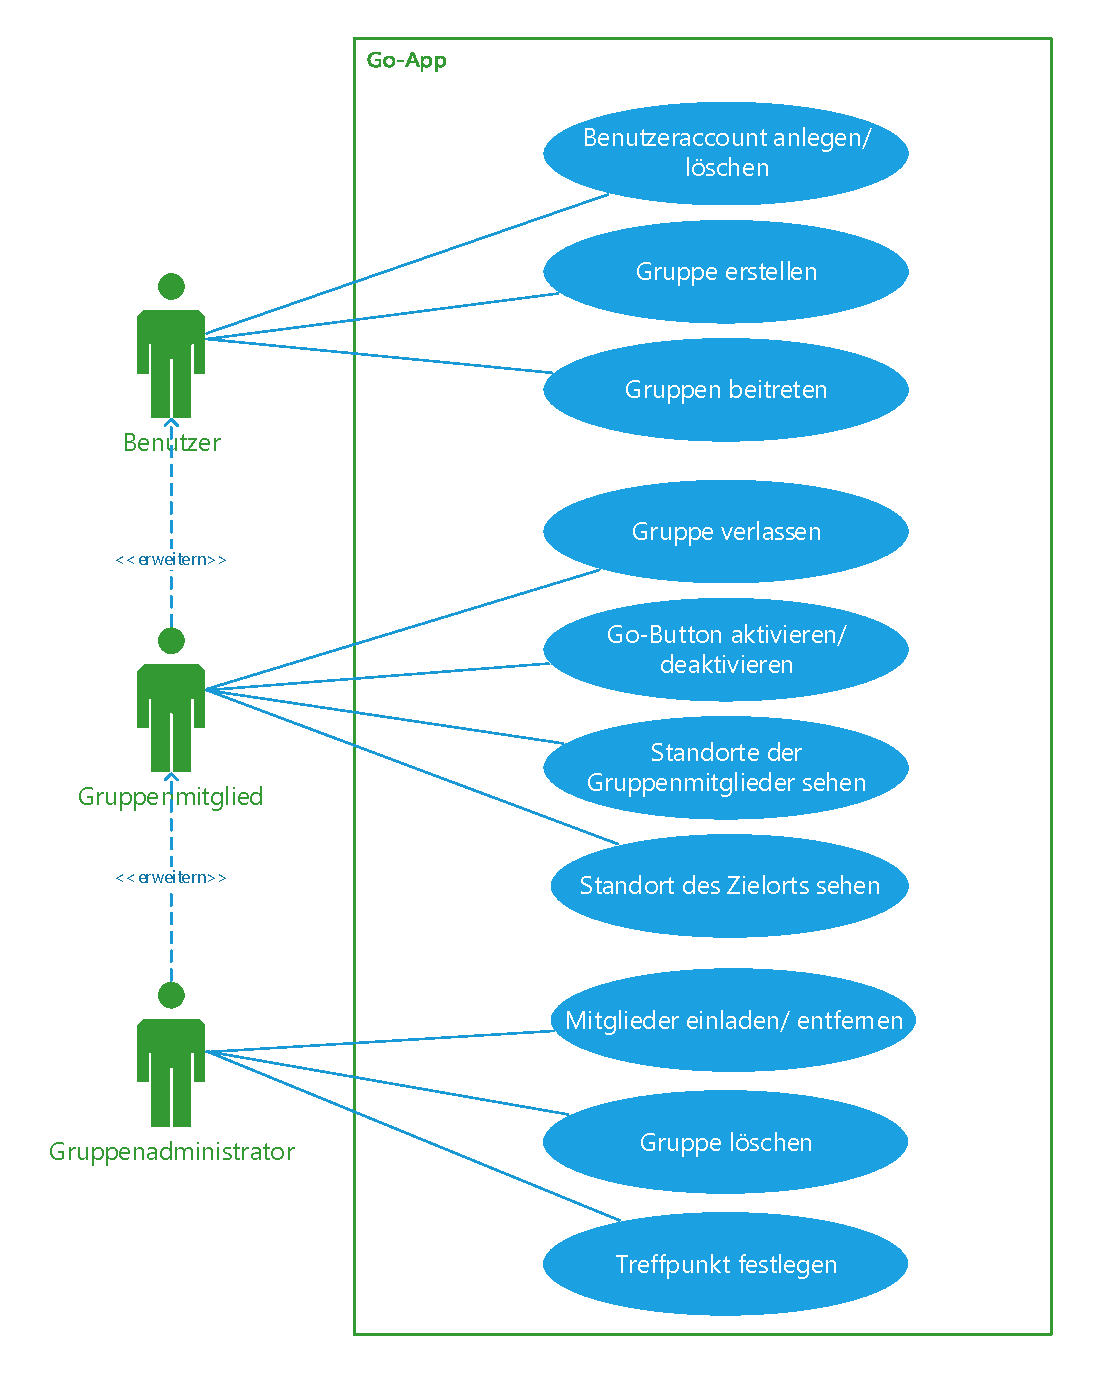
\includegraphics[scale=0.7]{resources/images/anwendungsfaelle/Anwendungsfalldiagramm.pdf}
	\centering
\end{figure}

\clearpage

\subsection{Wunschkriterien}
\begin{figure}[h]
	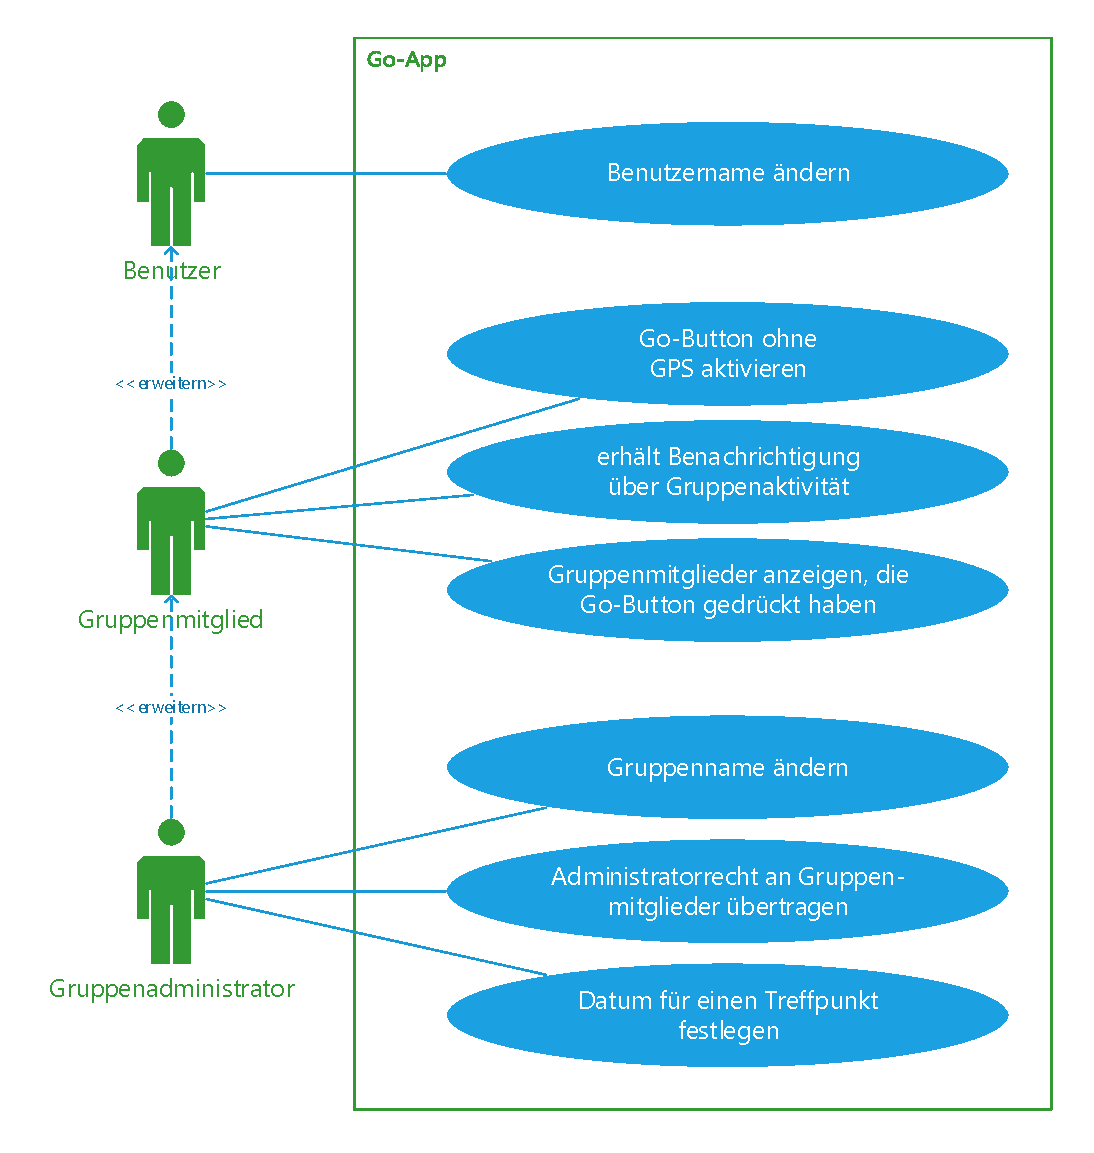
\includegraphics[scale=0.8]{resources/images/anwendungsfaelle/AnwendungsfalldiagrammWK.pdf}
	\centering
\end{figure}

\clearpage
